\documentclass[conference]{IEEEtran}
%
%% article_syscon.tex
%% V1.4
%% 2012/12/27
%% by Smail Rahmoun

%% Support sites:
%% http://www.michaelshell.org/tex/ieeetran/
%% http://www.ctan.org/tex-archive/macros/latex/contrib/IEEEtran/
%% and
%% http://www.ieee.org/

% Add the compsoc option for Computer Society conferences.
%
% If IEEEtran.cls has not been installed into the LaTeX system files,
% manually specify the path to it like:
% \documentclass[conference]{../sty/IEEEtran}


% Some very useful LaTeX packages include:
% (uncomment the ones you want to load)


% *** MISC UTILITY PACKAGES ***
%
%\usepackage{ifpdf}
% Heiko Oberdiek's ifpdf.sty is very useful if you need conditional
% compilation based on whether the output is pdf or dvi.
% usage:
% \ifpdf
%   % pdf code
% \else
%   % dvi code
% \fi
% The latest version of ifpdf.sty can be obtained from:
% http://www.ctan.org/tex-archive/macros/latex/contrib/oberdiek/
% Also, note that IEEEtran.cls V1.7 and later provides a builtin
% \ifCLASSINFOpdf conditional that works the same way.
% When switching from latex to pdflatex and vice-versa, the compiler may
% have to be run twice to clear warning/error messages.

% *** CITATION PACKAGES ***
%
\usepackage{cite}

% *** GRAPHICS RELATED PACKAGES ***
%
\ifCLASSINFOpdf
\usepackage[pdftex]{graphicx}
  % declare the path(s) where your graphic files are
  % \graphicspath{{../pdf/}{../jpeg/}}
  % and their extensions so you won't have to specify these with
  % every instance of \includegraphics
  % \DeclareGraphicsExtensions{.pdf,.jpeg,.png}
\else
  % or other class option (dvipsone, dvipdf, if not using dvips). graphicx
  % will default to the driver specified in the system graphics.cfg if no
  % driver is specified.
\usepackage[dvips]{graphicx}
  % declare the path(s) where your graphic files are
  % \graphicspath{{../eps/}}
  % and their extensions so you won't have to specify these with
  % every instance of \includegraphics
  % \DeclareGraphicsExtensions{.eps}
\fi


% *** MATH PACKAGES ***
%
\usepackage[cmex10]{amsmath}


% *** SPECIALIZED LIST PACKAGES ***
%
\usepackage{algorithmic}

% *** ALIGNMENT PACKAGES ***
%
\usepackage{array}

% *** SUBFIGURE PACKAGES ***
\ifCLASSOPTIONcompsoc
  \usepackage[caption=false,font=normalsize,labelfont=sf,textfont=sf]{subfig}
\else
  \usepackage[caption=false,font=footnotesize]{subfig}
\fi

% *** FLOAT PACKAGES ***
%
%\usepackage{fixltx2e}
%\usepackage{stfloats}
\usepackage{dblfloatfix}

% *** PDF, URL AND HYPERLINK PACKAGES ***
\usepackage{url}

% correct bad hyphenation here
\hyphenation{op-tical net-works semi-conduc-tor}

\begin{document}
\title{Using NSGA-II to compose model transformations alternatives }

\author{\IEEEauthorblockN{Smail Rahmoun}
\IEEEauthorblockA{Institute for Technological Research\\SystemX\\
Palaiseau France\\
Email: smail.rahmoun@irt-systemx.fr}
\and
\IEEEauthorblockN{Etienne Borde\\ and Laurent Pautet}
\IEEEauthorblockA{TELECOM Paristech Institut\\
LTCI-UMR 5141\\
Paris, France\\
Email: firstname.name@telecom-paristech.fr}}

\maketitle

\begin{abstract}
The size and complexity of modern systems is rapidly increasing. Meanwhile, the ability to understand and maintain such systems is decreasing almost as fast.
Model Driven Engineering (MDE) promotes the automation of design activities by means of model transformations, enabling to cope with systems complexity. However, the design space produced by the composition of these model transformations is difficult to explore automatically. The main reason that make this exploration difficult is the size of the design space : the number of possible design choices grows exponentially with the number of model transformation alternatives.
This paper presents a MDA approach for design space exploration to deal with the ever-growing challenge of designing complex embedded systems. This approach allows the system architects to automatically select the most adequate model transformations compositions by using multi-objectives optimization evolutionary algorithms (MOEA) mechanisms.

%modeling solution for their application, platform, and mapping between application and platform, in an integrated and simultaneous way and at a very early design stage, before system synthesis and code generation have been performed. 



%multi-objective optimization evolutionary algorithms which is known to be an important tool for design decision making support.

%The design of safety-critical systems becomes one of the most interesting challenges in modern systems engineering. It requires system architects to address a large number of non-functional properties related to performance, reliability, availability and temporal performance. Moreover, these non-functional properties often conflict with each other, for instance, improving system performance often needs more powerful hardware components, which increases the production cost and power consumption in the meantime. 



%and model transformation strategies to identify a sufficient set of design alternatives. This approach will reduce development costs and improve the quality of the final system, because an automated and systematic search will identify more and better design alternatives.



%In this paper, we propose an approach which can analyse a given system architecture, propose design alternatives to it by using model transformations, and do architecture optimization by using some evolutionary algorithms to improve its non-functional properties in an automatic way.
\end{abstract}


%This paper proposes to use multi-objective optimization evolutionary algorithms and model transformation strategies to identify a sufficient set of design alternatives. This approach will reduce development costs and improve the quality of the final system, because an automated and systematic search will identify more and better design alternatives.



% no keywords

\IEEEpeerreviewmaketitle

\section{Introduction}
Nowadays, modern systems become more and more large and complex and therefore more difficult to develop and maintain. For example, embedded critical systems which are often built to accomplish specific functionalities, can integrate thousands of buses, software and hardware components. To guarantee properties such as safety, availability and robustness makes the design of these systems very challenging and complicated.

Model Driven Engineering (MDE) proposes the use of models as the key assets in the development of such systems, and hence all sorts of model modifications are needed. In this way, model transformations become one of the basic building blocks of MDE. Even though MDE is being successfully applied in many scenarios, it still needs appropriate mechanisms to handle the development of complex, large-scale systems. One such mechanism is a facility to make transformations reusable, so that we can apply them to different contexts. In this work, we use generic model transformation to model design alternatives of the system. This process will help us to predict NFP of a system before it development\cite{1291833}. This prediction can be exploited to drive decisions about which components should be used and how they should be connected so as to meet the NFP imposed on the design.

Moreover, an issue in modeling the NFP of a system is that, the NFP could conflict\footnote{improving one property can have a negative impact on other properties} with each other. For example, improving the availability of a service is often done by replication of the service, which causes the increasing of the response time of these services\cite{Yu:2001:CLA:502059.502038}. Developing a system that satisfies at best all its NFP simultaneously is often not possible : improving a NFP of a system can deteriorate another NFP. As a consequence, system architects have to come up with several design alternatives and select the optimal solution (Pareto optimal solutions) from all feasible alternatives through the trade-off analysis regarding all NFP\cite{Coello98acomprehensive}.

In order to obtain the set of Pareto optimal alternatives, some advanced multi-objective optimization evolutionary algorithms (MOEA) have been proposed. These algorithm apply some fitness evaluations and generic operators of variation. Thus, they are applicable to search spaces (e.g. design space) taking into account domain specific characteristics of the problem (e.g. prediction of NFP). MOEA also provides selection operators which guide the search towards interesting regions of the search space by (i) favorizing non-dominated solutions : where a solution x1 is dominated by another solution x2 , if x2 matches or exceeds x1 in all objectives; (ii) finding a diverse set of solutions on the Pareto front.

Our approach, consists in improving the NFP of an architecture design through a generic method using model transformations compositions and advanced MOEA. This method will automate the search for optimal compositions from all feasible alternatives. More specific, beginning with some initial architecture that specifies a set of NFP, design alternatives are generated by applying model transformation compositions\cite{Jouault:2005:TMA:2153686.2153705}. To get the non-dominated alternatives, model transformation rules enter into a meta-heuristic loop. That is, we generate transformation rules alternatives (TRA) through some genetic operations such as mutation and crossover. The models transformed by the selected TRA are evaluated and corresponding multiple NFP criteria of interests are obtained after application of transformations in order to obtain more precise analysis.

The reminder of this paper is organized as follows. Section~\ref{Problem} is dedicated to the problem statement. Section~\ref{Approach} gives an overview  of our approach. While Section~\ref{Adapting} details our approach. Section~\ref{Related} presents the related work.
%The remainder of this paper is organized as follows. Section~\ref{Problem} is dedicated to the problem statement. Section~\ref{Approach} gives an overview  of our approach. While Section~\ref{Adapting} details our approach. Section~\ref{Related} presents the related work. Finally, conclusions and perspectives are given in Section~\ref{Conclu}.

\section{Problem}
\label{Problem}
During the design of a safety-critical system, it is useful to model non functional properties (NFP), such as reliability, availability or temporal performances, already in early stages of the development process. Early NFP modeling enables the developer of the system to make design decision based on analyses and simulations. But, one major difficulty is that these NFP can be in conflict with each other, that is, improving one NFP can have a negative impact on others. To construct a system that fulfils all its NFP simultaneously is often not possible. As a consequence, system architects have to consider several design alternatives, and identify a solution that fulfils most NFP (an optimal solution) from all feasible alternatives. 

A possible solution to this issue is to implement these design alternatives in a way that they can be seen as design patterns. Where each pattern implement a well-known architectural solution which fulfils a set of NFP. To formalize these design patterns in a way that allow their reuse in different projects or products we implement them as model transformations.

%These design patterns are implemented as model transformations. It  which allows us to applied them to various sets of NFP

%improving a set NFP, and solving the conflict between these NFP.  Model transformations are usually defined to be generic such as design patterns which allows us to applied them to various sets of NFP.


%A set of model transformations that implement refinements or improvements of the source model, each of them focusing on increasing the satisfaction of a given goal (reducing power consumption, increasing availability, etc.). These model transformations can be seen as design patterns, each of them implementing a well-known solution to a given quality objective.


%A possible solution to this issue is to formalize design alternatives so they can be reusable in different products or projects (i.e. by using model transformation techniques). After the formalization step, explore the design space to identify the set of optimal model transformation alternatives : solutions that fulfils most NFP.

The second challenge in this work comes from the size of the design space to explore in order to study such NFP trade-offs. With a complex system and a larger design space, it is almost impossible for software architects to find optimal architecture designs. The exploration of such design space can be very difficult to do manually and error-prone. To overcome this issue, we propose an approach to assist architects throughout the modeling phase and automate the design space exploration by using existing multiple objective evolutionary algorithms (MOEA).

Moreover, using MOEA to deal with mode transformations alternatives can be challenging. We have (i) to generalize the architecture design problem as a multiple objective optimization problem; (ii) select the more suitable evolutionary algorithm to solve this optimization problem; and (iii) adapting the notions of model transformation compositions to this evolutionary algorithm.

\section{Using evolutionary algorithms for identifying good design alternatives}
\label{Approach}
Figure~\ref{IS} graphically illustrates the approach proposed in this paper by showing the process underlying it. As can be seen in Figure~\ref{IS}, the process starts with an initial input software architecture which could be designed by software architects by using some architecture design language\cite{Medvidovic}. After that, this architecture model is transformed into a set of alternative architecture models (more detailed models) which fulfils a set of competing NFP such as reliability, availability and response time. To solve the trade-off between NFP we expressed the architecture alternatives as design patterns implemented by means of model transformations and compositions techniques. The final step in Figure~\ref{IS} consists in exploring the design space composed of all model transformation compositions and select which transformation fulfil at best the NFP of the system. This step is done by using an advanced evolutionary algorithm.

\begin{figure}[!t]
\centering
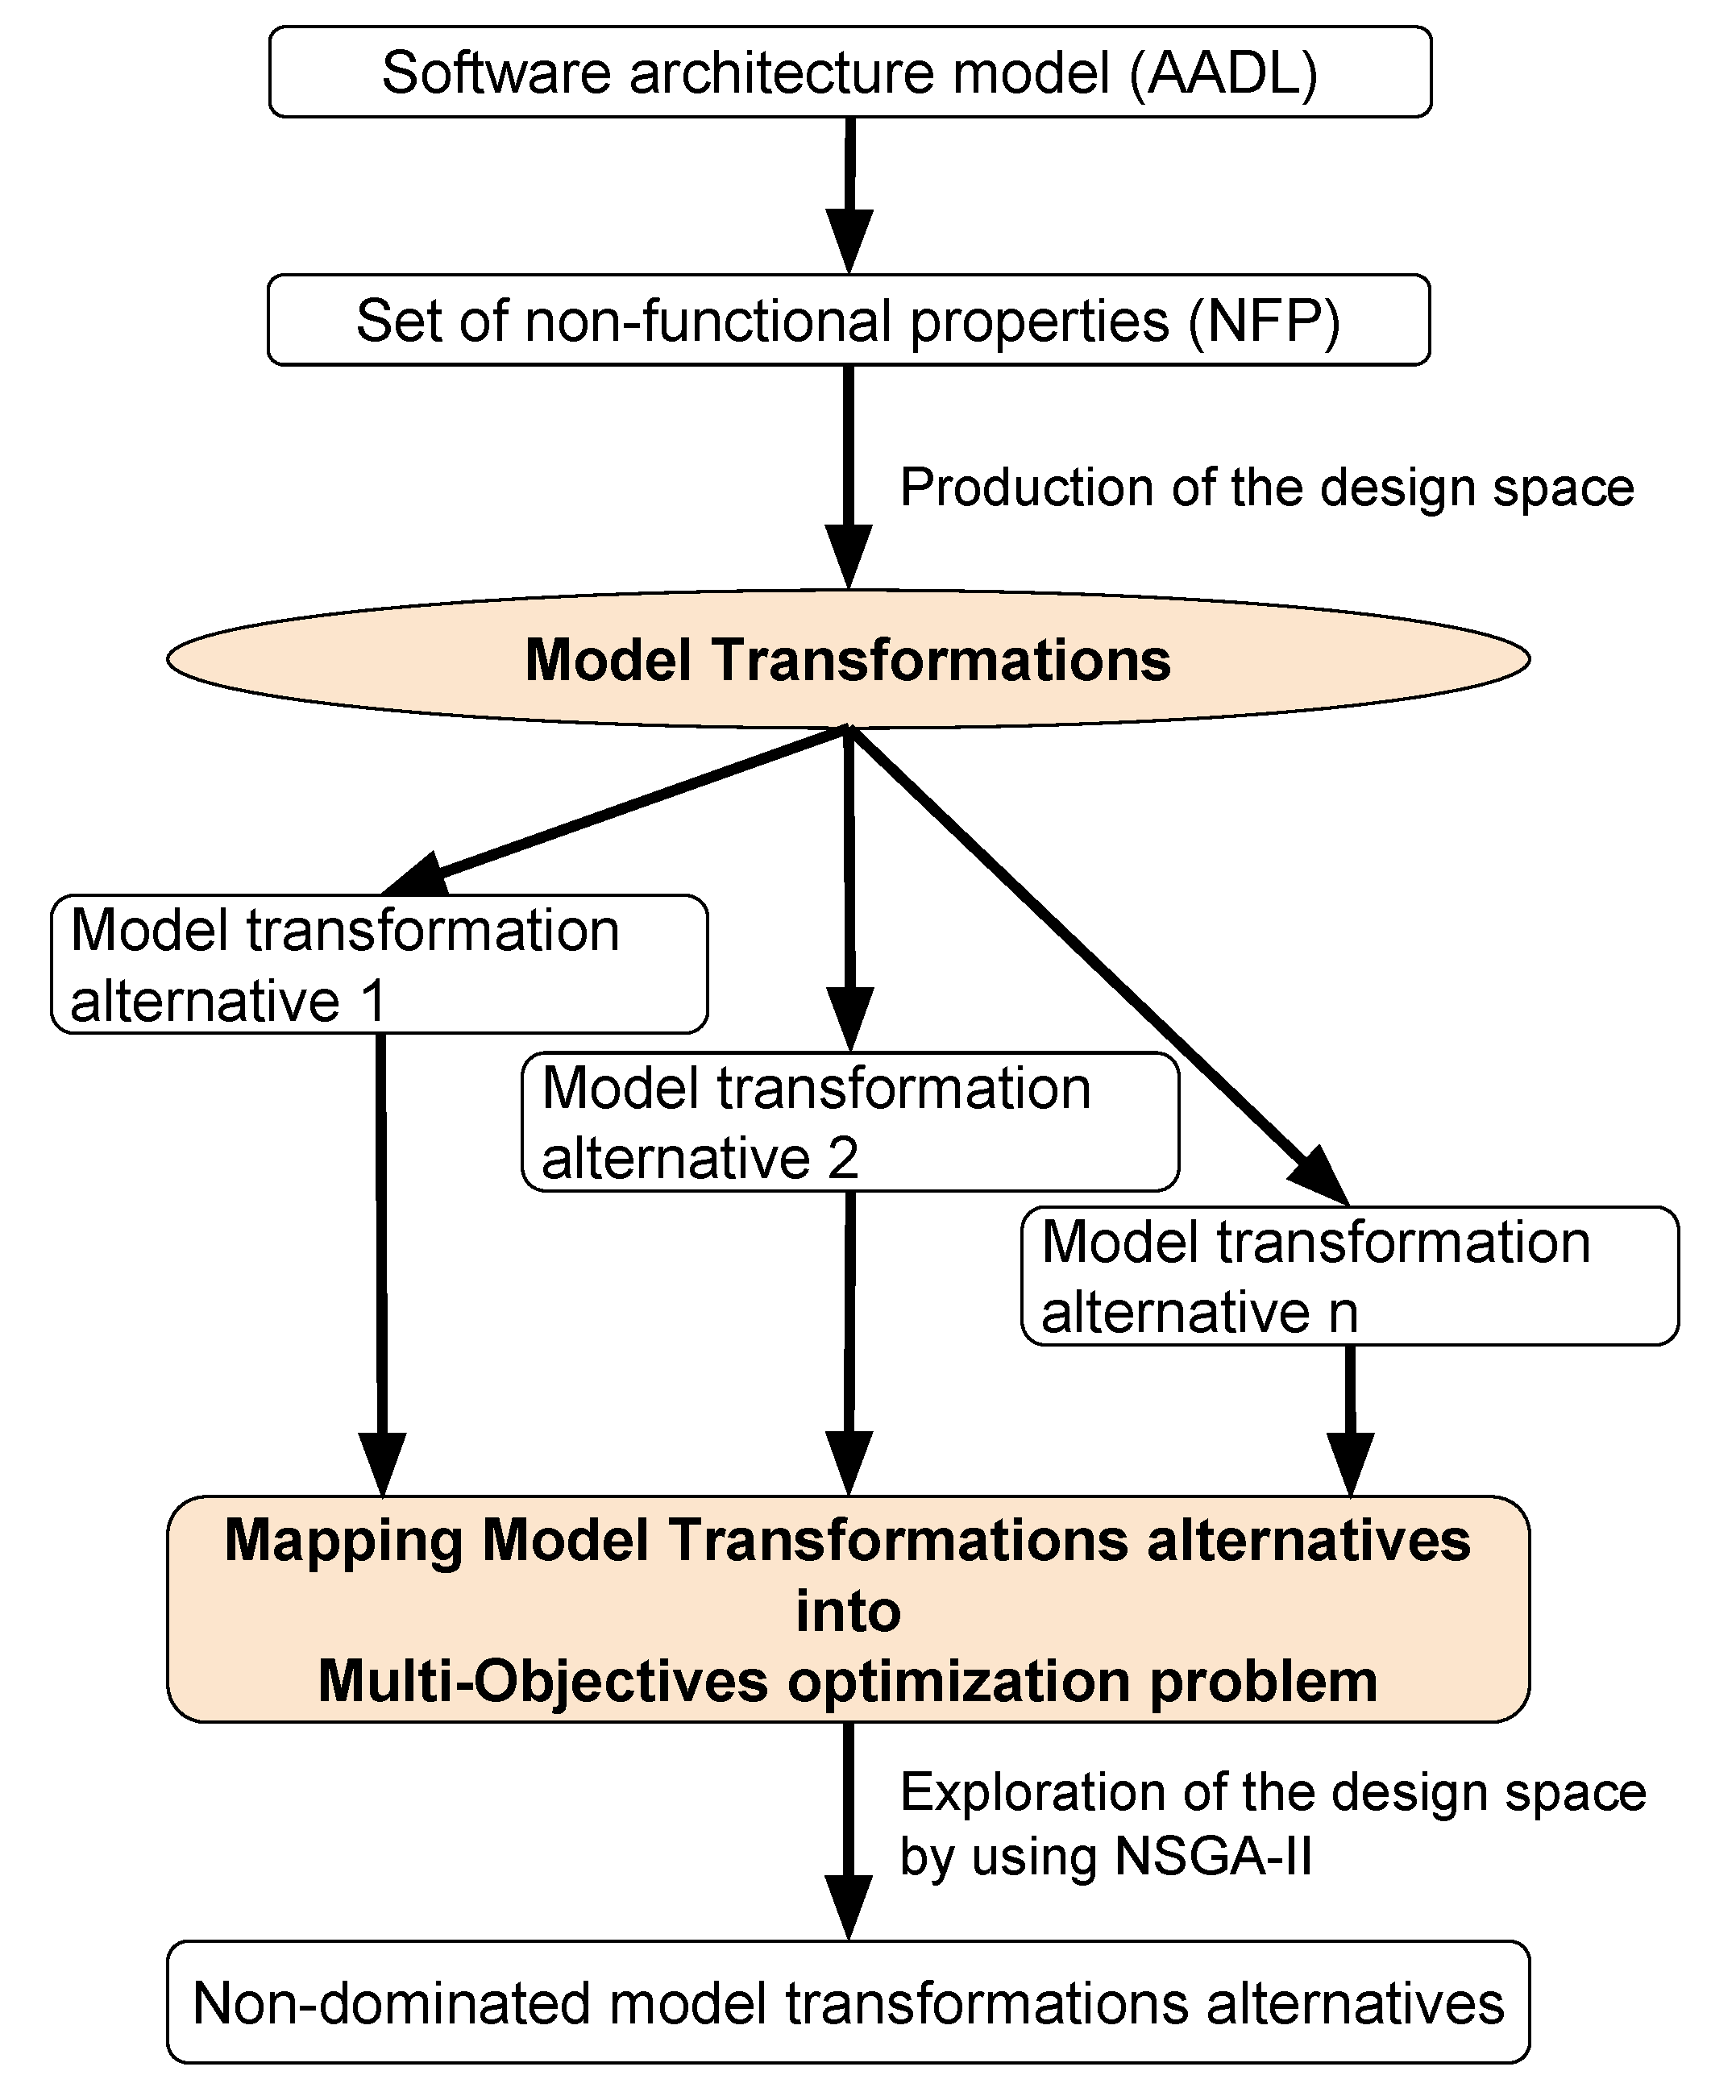
\includegraphics[width=3.49in]{IDMT.pdf}
\caption{Overview of the identification step}
\label{IS}
\end{figure}

\subsection{System architecture modelisation}
%For software architecture modeling step, as a natural extension of previous work RAMSES and  we choose to use AADL (Architecture Analysis & Design Language) as the underlying architecture description language.

Since our application domain is embedded systems, we have chosen AADL (Architecture Analysis \& Design Language) as the underlying architecture description language. AADL has been designed on the foundation of the architecture description language MetaH and its goals are (i) specification of quality analysis (e.g. safety); and (ii) design architectures for complex embedded systems. It offers a standardized semantics, mostly expressed using natural language and the components are composed hierarchically according to standardized composition rules. AADL also allows the designers to expand model by defining new property sets in their own specific way. The other reason of choosing AADL is to integrate our work in an existing framework RAMSES\footnote{Refinement of AADL Models for the Synthesis of Embdded Systems. \url{http://penelope.enst.fr/aadl/wiki/Projects}} which apply selection of design alternatives.

\subsection{Multi-Objective Genetic Algorithm}
In order to deal with the multi-objective nature of our problem (which model transformation achieve the best possible trade-off among NFP) we use MOEA. 
Among the many MOEAs that have been proposed in the literature : NSGA-II\cite{Deb:2002:FEM:2221359.2221582}, SPEA2\cite{Zitzler01spea2:improving}, IBEA\cite{Zitzler04indicatorbasedselection}, only one have been considered in this work, namely NSGA-II (Non-dominated Sorting Genetic Algorithm). It was proposed in the early 90's and still considered today as one of the state-of-the-art MOEA for its robustness across a variety of application domain.

\subsection{NSGA-II}
NSGA-II is an improved version of NSGA\cite{Srinivas94multiobjectiveoptimization} (Non-dominated sorting genetic algorithm). It inherited the non-dominance concept from NSGA and showed three innovations, (i) a crowding approach for diversity preservation; (ii) an elitism operator that helps in significantly speeding up the performance of the genetic algorithm (fast non-dominated sort); and (iii) an objective-wise distance computation. 

\begin{figure}[!t]
\centering
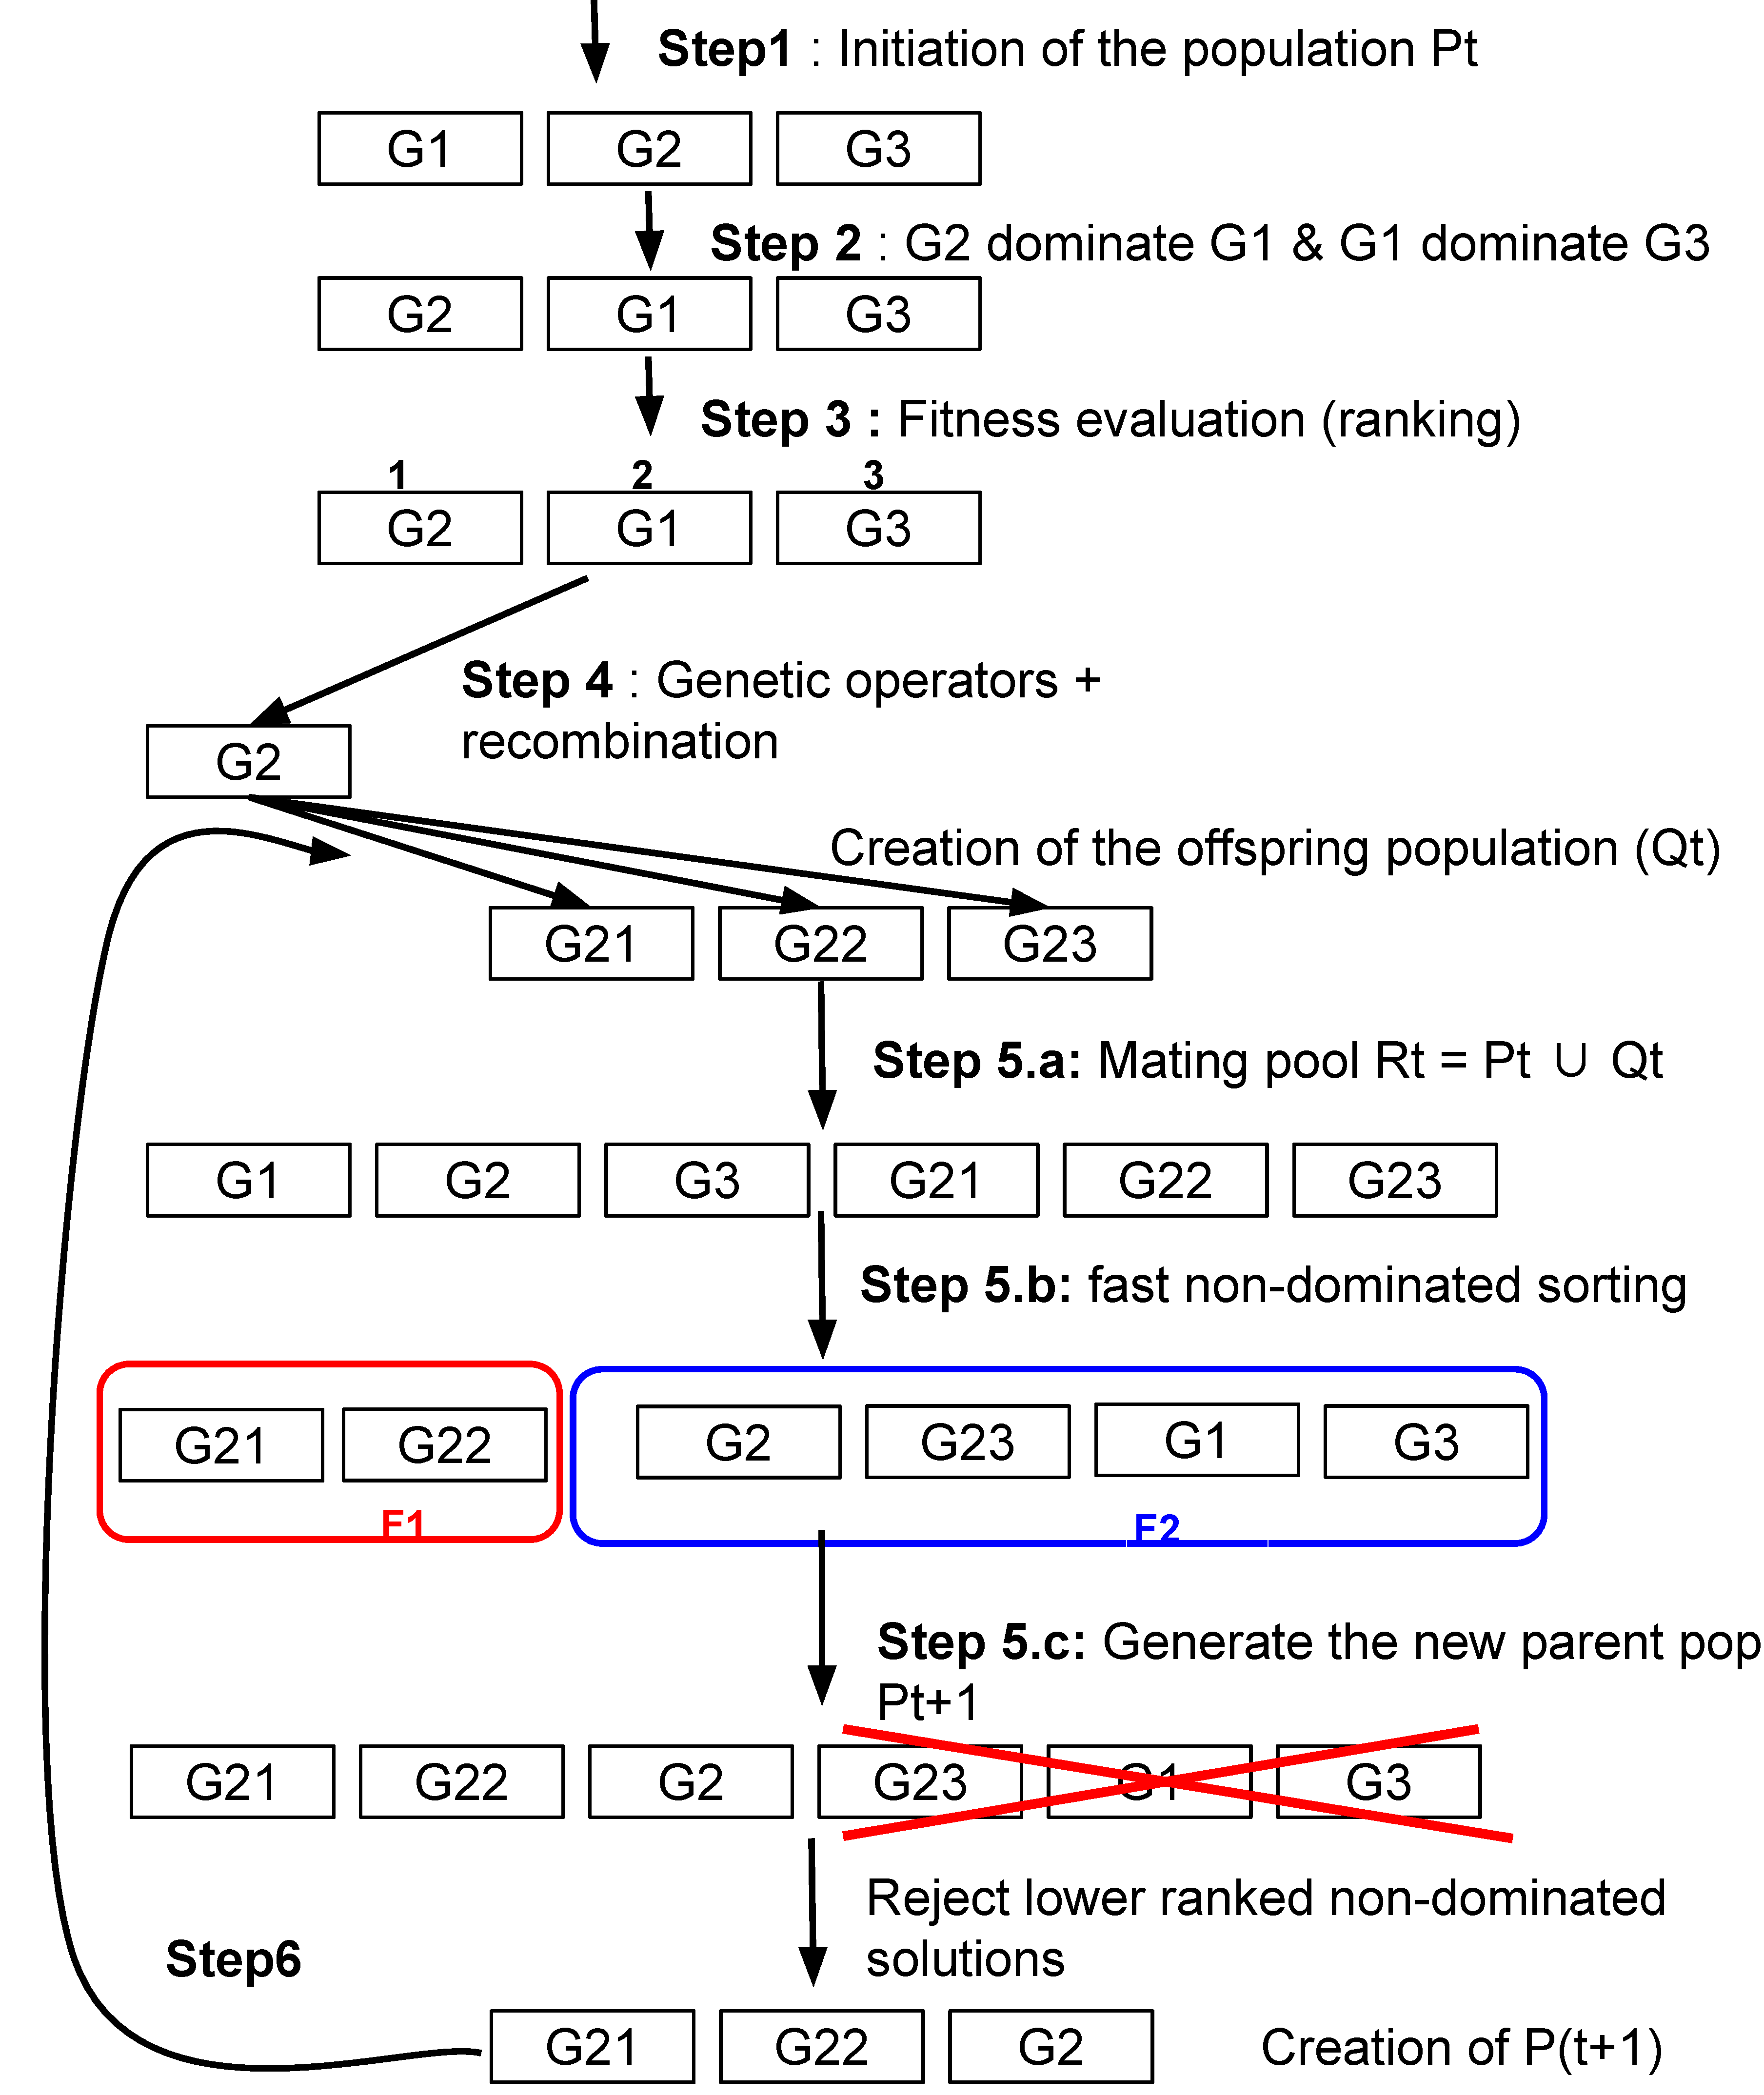
\includegraphics[width=3.49in]{NSGAII.pdf}
\caption{Schema of the NSGA-II algorithm}
\label{nsgaii}
\end{figure}

Figure~\ref{nsgaii} gives an overview of how to use NSGA-II to automate the exploration of complex systems design space. The steps of this algorithm are as follow :

\begin{enumerate}
\item Initially, Create a random parent population $P_{0}$ composed of N genomes (N = 3 in Figure~\ref{nsgaii}).
\item Sort the current population based on a non domination criterion (e.g. reliability, availability and response time).
\item For each non-dominated solution, assign a fitness (rank) equal to its non-domination level (1 is the best level, 2 is the next best level, and so on).
\item Create a child population $Q_{0}$ of size N using binary tournament selection, recombination, and mutation operators.
\item From the first generation onwards, creation of each new generation constitutes the following steps :
	\begin{enumerate}	
	\item Create the mating pool $R_{t}$ of size 2N by combining the parent population $P_{t}$ and the child population $Q_{t}$.
	\item Sort the combined population $R_{t}$ according to the fast non-dominated sorting procedure to identify all non-dominated fronts $(F_{1} ,F_{2},...,F_{k})$.
	\item Generate the new parent population $P_{t}+1$ of size N by adding non-dominated solutions starting from the first ranked non-dominated front $F1$ and proceeding with the subsequently ranked non-dominated fronts $F_{1} ,F_{2}, . . . ,F_{k}$, till the size exceeds N (Figure~\ref{nsgaii}). This means that the total count of the non-dominated solutions from the fronts $F_{1} ,F_{2}, . . . ,F_{k}$, exceeds the population size N. Now, in order to make the total count of the non-dominated solutions equal to N, it is required to \textbf{reject} some of the lower ranked non-dominated solutions from the last $Fkth$ front. This is achieved through a sorting process based on the crowding distance assigned to each solution contained in the $F_{k}th$ non-dominated front. Thus, the new parent population $P_{t}+1$ of size N is constructed.
	\item Perform the selection, crossover and mutation operations on the newly generated parent population $(P_{t}+1)$ to create the new child population $(Q_{t}+1)$) of size N (Figure~\ref{nsgaii}).
	\end{enumerate}
\item Repeat Step 5 until a stopping criterion is met (e.g. maximum number of generations is reached).

\end{enumerate}

\section{Compose model transformation alternatives by using NSGA-II}
\label{Adapting}

In this paper we propose a generic method to automate the search of optimal architectures (which fulfil at best the NFP of the system) from the design space. To represent the design space (set of architecture alternatives) we use model transformations compositions. The exploration step is done by using the NSGA-II algorithm.

\subsection{Model transformations languages}
In general, model transformations are grouped into two main categories of model transformation languages : (i) rule-based transformation languages, or (ii)
imperative transformation languages. We used in our work the first category of languages since it express model transformation logics in a way that is easy to interpret and \textbf{adapt} in other methods (in this paper MOEA). To be continued by giving more explanations about rule-based transformations languages

%Examples of rule-based transformation languages ATL (for Atlas Transformation Language) and QVT-R (for ).


%such as ATL and QVT-R, are of great interest in our context since they express model transformation logics in a way that is easy to interpret and adapt. Indeed, modifying the pattern matching part of a transformation rule is sufficient to modify the set of elements this rule applies to. In addition, superimposition helps to combine different sets of rules [15]. Contrasting with rule-based formalisms, the adaptation of imperative transformation languages requires a deep understanding of the control flow graph that leads to the execution of one or another transformation. Model transformations we deal with in this paper are endogenous (AADL[13] to AADL model transformations) in order to refine or improve the architecture of an embedded system while representing the result of this refinement in an analyzable model (using AADL as an output language).

\subsection{Genome representation}
The first step of our work consists in applying the definition of the multi-objective optimization problem on our architecture design problem. Where the population to optimize or the design space represent a set of architecture alternatives and the objectives functions are $f_{1}:$ reliability, $f_{2}:$ availability and $f_{3}:$ response time. The architecture alternatives are formalized in a way that allow their reuse in different projects or products. To do so, we use model transformations methods. An issue in using such methods is their complexity : how to identify which elements of the input architecture model transformation alternatives can be applied. To ease the development and maintenance of such model transformations, we propose to use a rule-based transformation language and composition mechanisms. These languages define rules which define the mapping from source elements (elements of the software architecture) to target element (architecture alternative). 

In our approach we call these rules TRA (Transformation Rules Alternatives). They represent the genomes to optimize in our multi-objective problem. Figure~\ref{genome} gives an overview of these genomes. Each genome $G_{i}, i \in {1,2,...,n}$ is composed of a set of TRA $(G = {TRA_{i}, i \in {1,2,...n}})$. Each $TRA_{i}$ is, in turn, encoded as a pair $TRA_{i} = <Elements_{i},Rule_{i}>$ where $Elements_{i} (i ={1,2,...,n})$ is a list of elements from the input model, and $Rule_{i} (i ={1,2,...,n})$ is a transformation rule which can be applied to $Elements_{i}$.


\begin{figure}[!t]
\centering
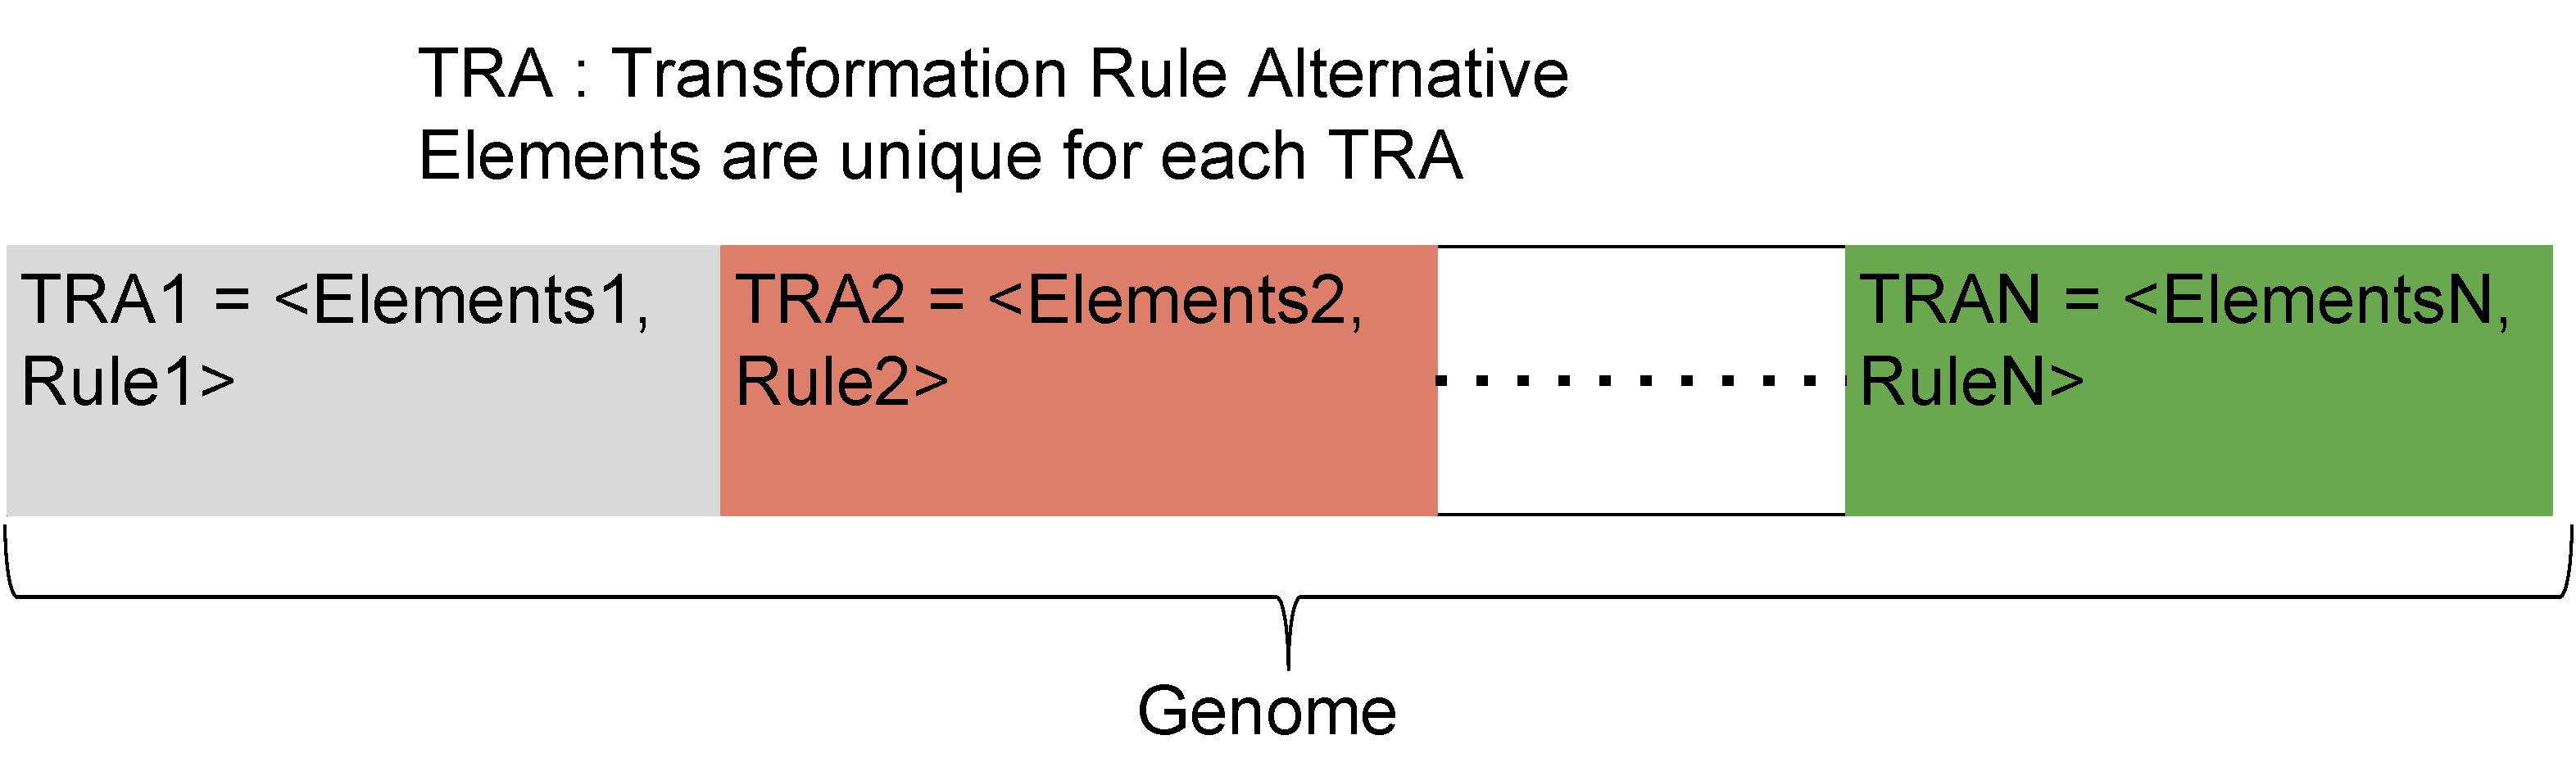
\includegraphics[width=3.49in]{genome.pdf}
\caption{Genome overview}
\label{genome}
\end{figure}

\subsection{Genome evaluation}
In each generation, the fitness of every genome in the population is evaluated. The fitness is usually the value of the objective function in the optimization problem being solved. We defined in our work one fitness function corresponding to three objectives reliability, availability and response time.
The aim of our work is to maximize these three objectives. 

The more fit genomes are stochastically selected from the current population, and each genome is modified (recombined and possibly randomly mutated) to form a new generation.

%\subsection{Adapting NSGA-II To explore the design space}
%The second step of our approach consists in (i) the exploration of the design space (composed of the set of genomes described above); and (ii) selection of the optimal genomes. This step is realised by adapting the concepts of the NSGA-II algorithm to our design problem. To do so, we use the same algorithm as described previously. Except that each genome is represented by a set of TRA.

\subsection{Genetic operators definition}
In NSGA-II, in each iteration, the N genomes selected from the previous generation are used to create new N genomes using genetic operators. This improves the existing solutions by mixing their genetic material (crossover) and/or by creating new material (mutation). Before applying the operators, the solutions are selected according to their fitness values, see Figure~\ref{nsgaii}. In our work, binary tournament selection, crossover and mutation operators are used.

\subsubsection{\textbf{Binary tournament selection}}
This operation consists of choosing some genomes at random in the population, and selecting the fittest two for reproduction. The selection criteria are the rank of the containing front and the crowding distance for solutions within the same front. Several tournaments are run to produce the N needed genomes.

Figure~\ref{binary} illustrates this operation. On this figure, we suppose we have four genomes (G1,G2,G3,G4) and we apply two tournaments to produce the needed genomes. The final genomes of the competition will always be the fittest genomes in the population. The more successful the genome is in competition, the more often that genome is expected to appear in the mating pool (In Figure~\ref{binary} the fittest genome is G4).

\begin{figure}[!t]
\centering
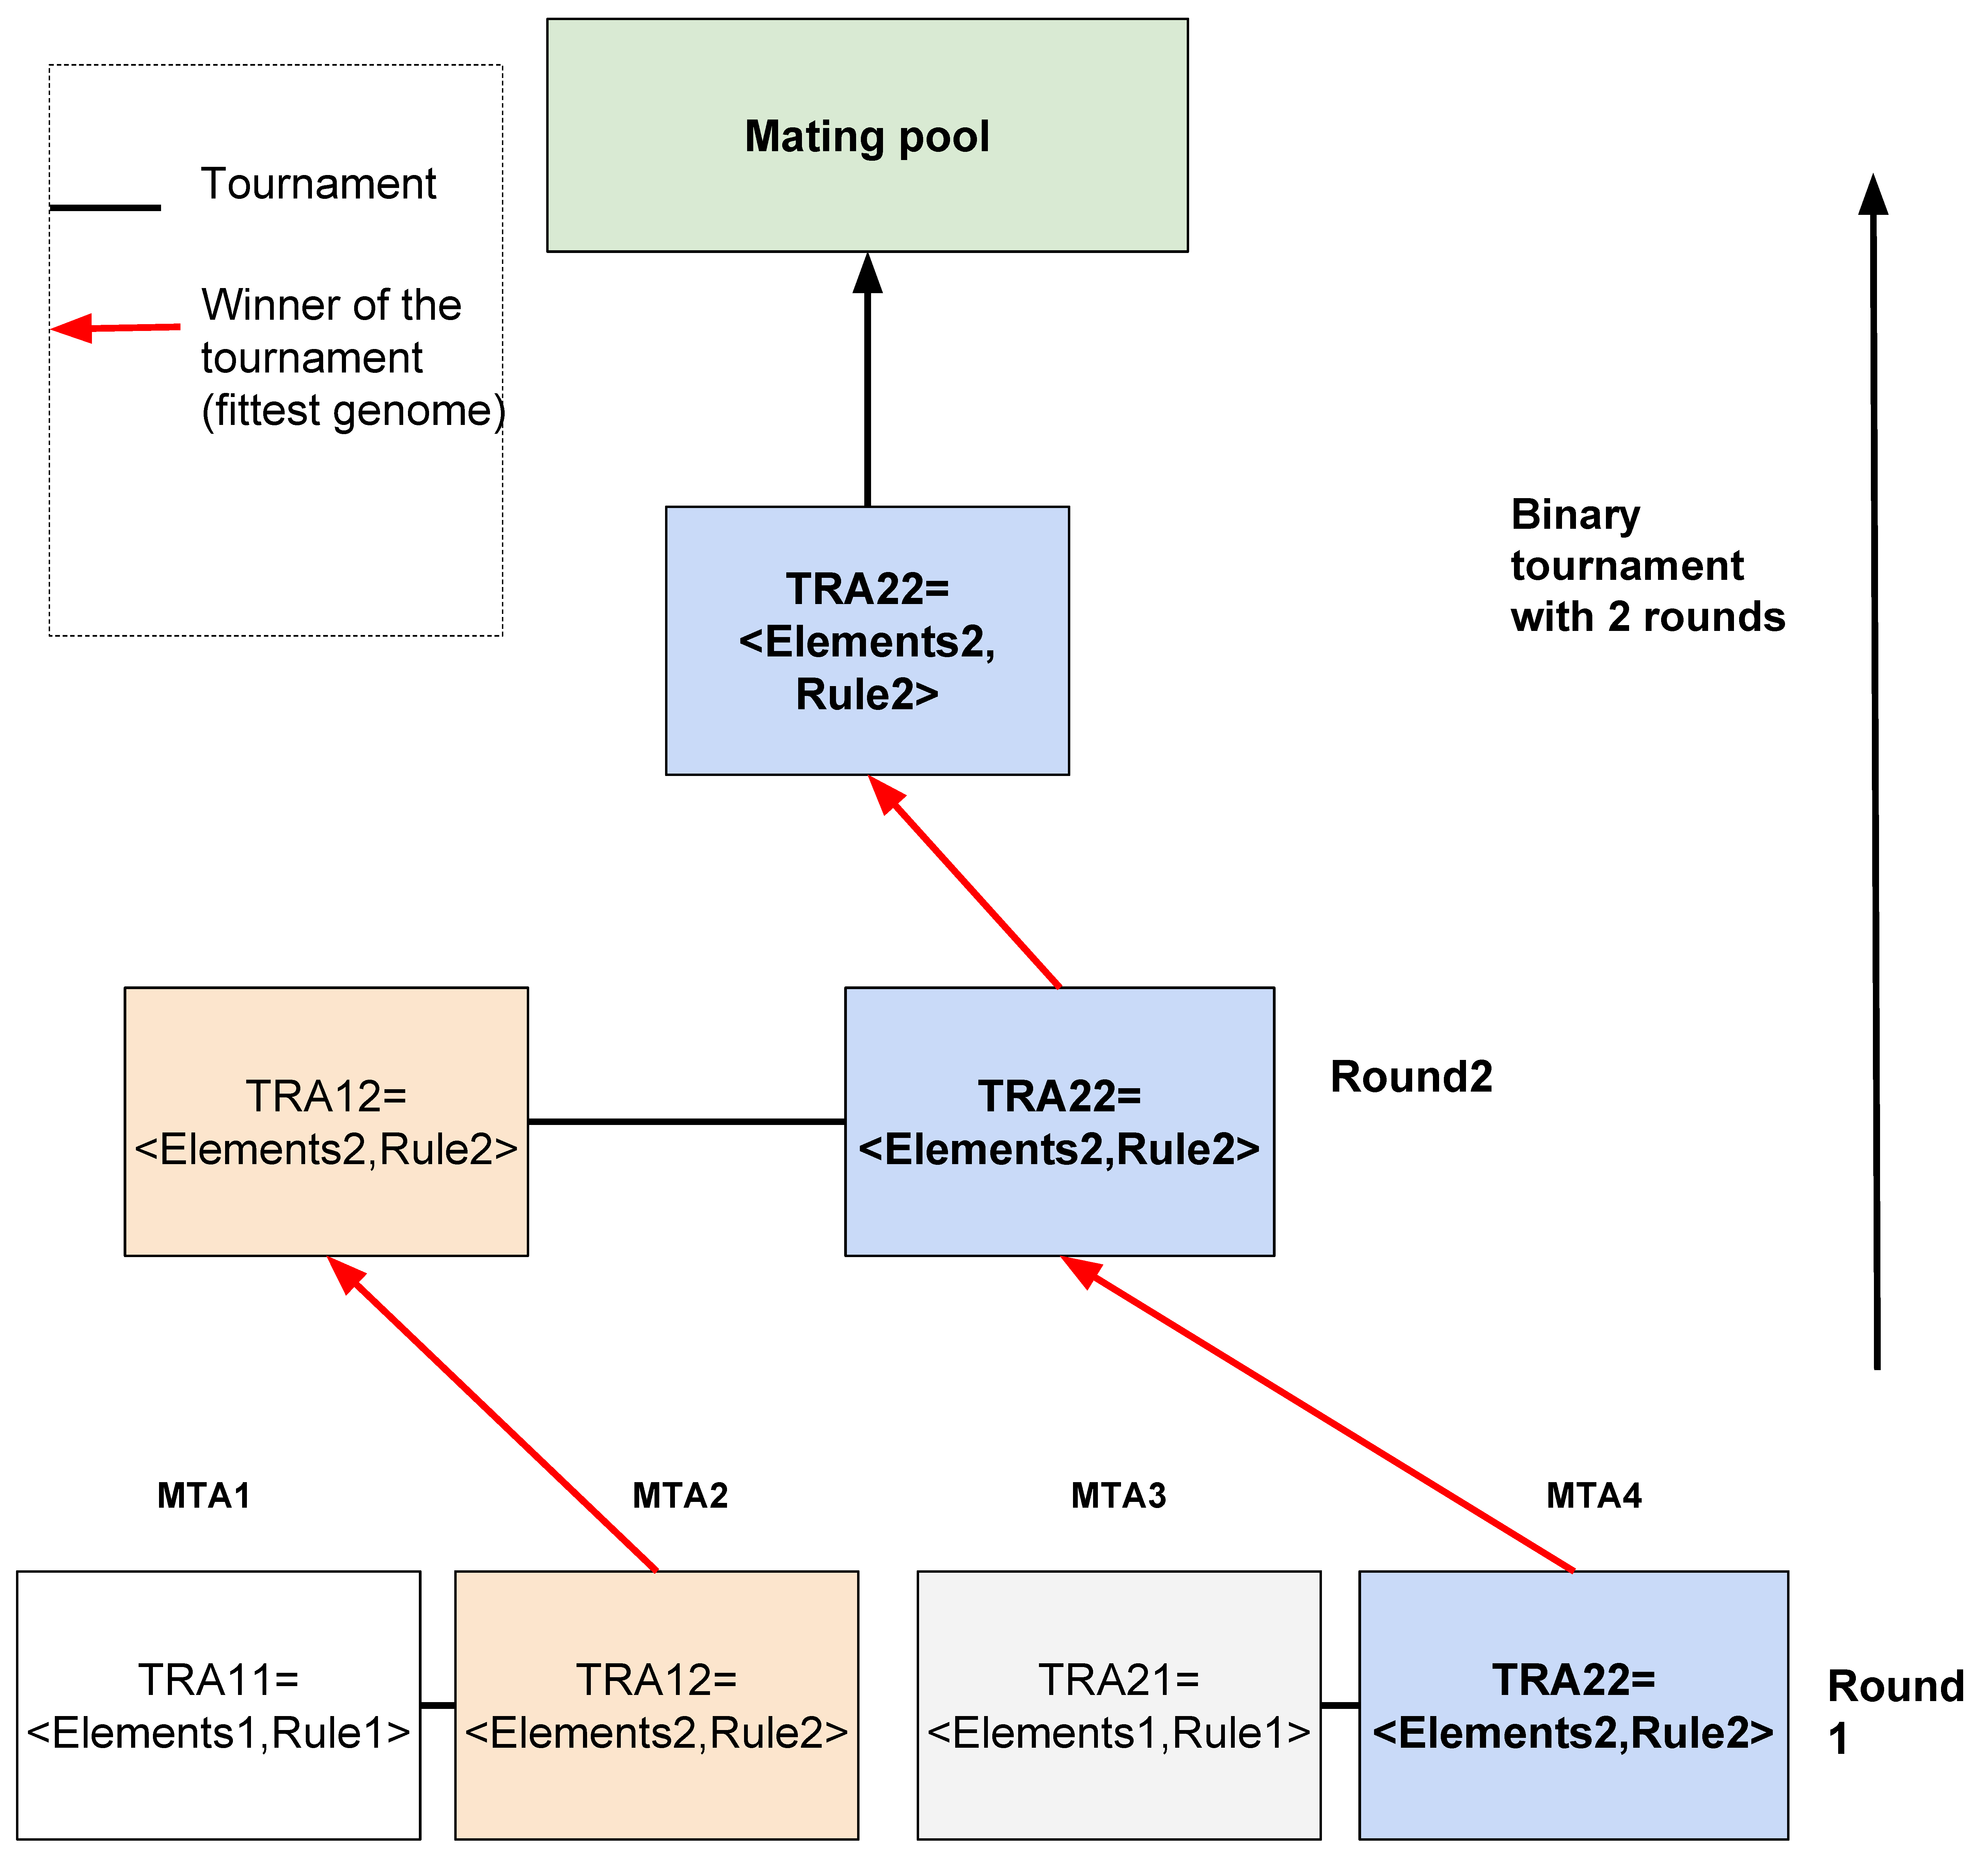
\includegraphics[width=3.49in]{bt.pdf}
\caption{Tournament Competition between Genomes}
\label{binary}
\end{figure}


\subsubsection{\textbf{Crossover}}
The crossover consists of producing new genomes from the existing ones. When two genomes are selected using the binary tournament selection, two offspring solutions are created, with a given crossover probability, by exchanging parts of the parent genomes. This consists in randomly selecting a cut point in the genome vector, and all the target fragments beyond that point in either parent are swapped between the two parents.

Figure~\ref{crossover} illustrates the result of applying the crossover operator to two parent genomes G1 and G2 respectively composed of \{TRA11,TRA12,TRA13\} and \{TRA21,TRA22,TRA23\} to produce a new genome G3. As can be seen in Figure~\ref{crossover}, this operator combines G1 and G2 by selecting a single point on the genome and swapping the genes between the two genomes that lie beyond this point. 

\begin{figure}[!t]
\centering
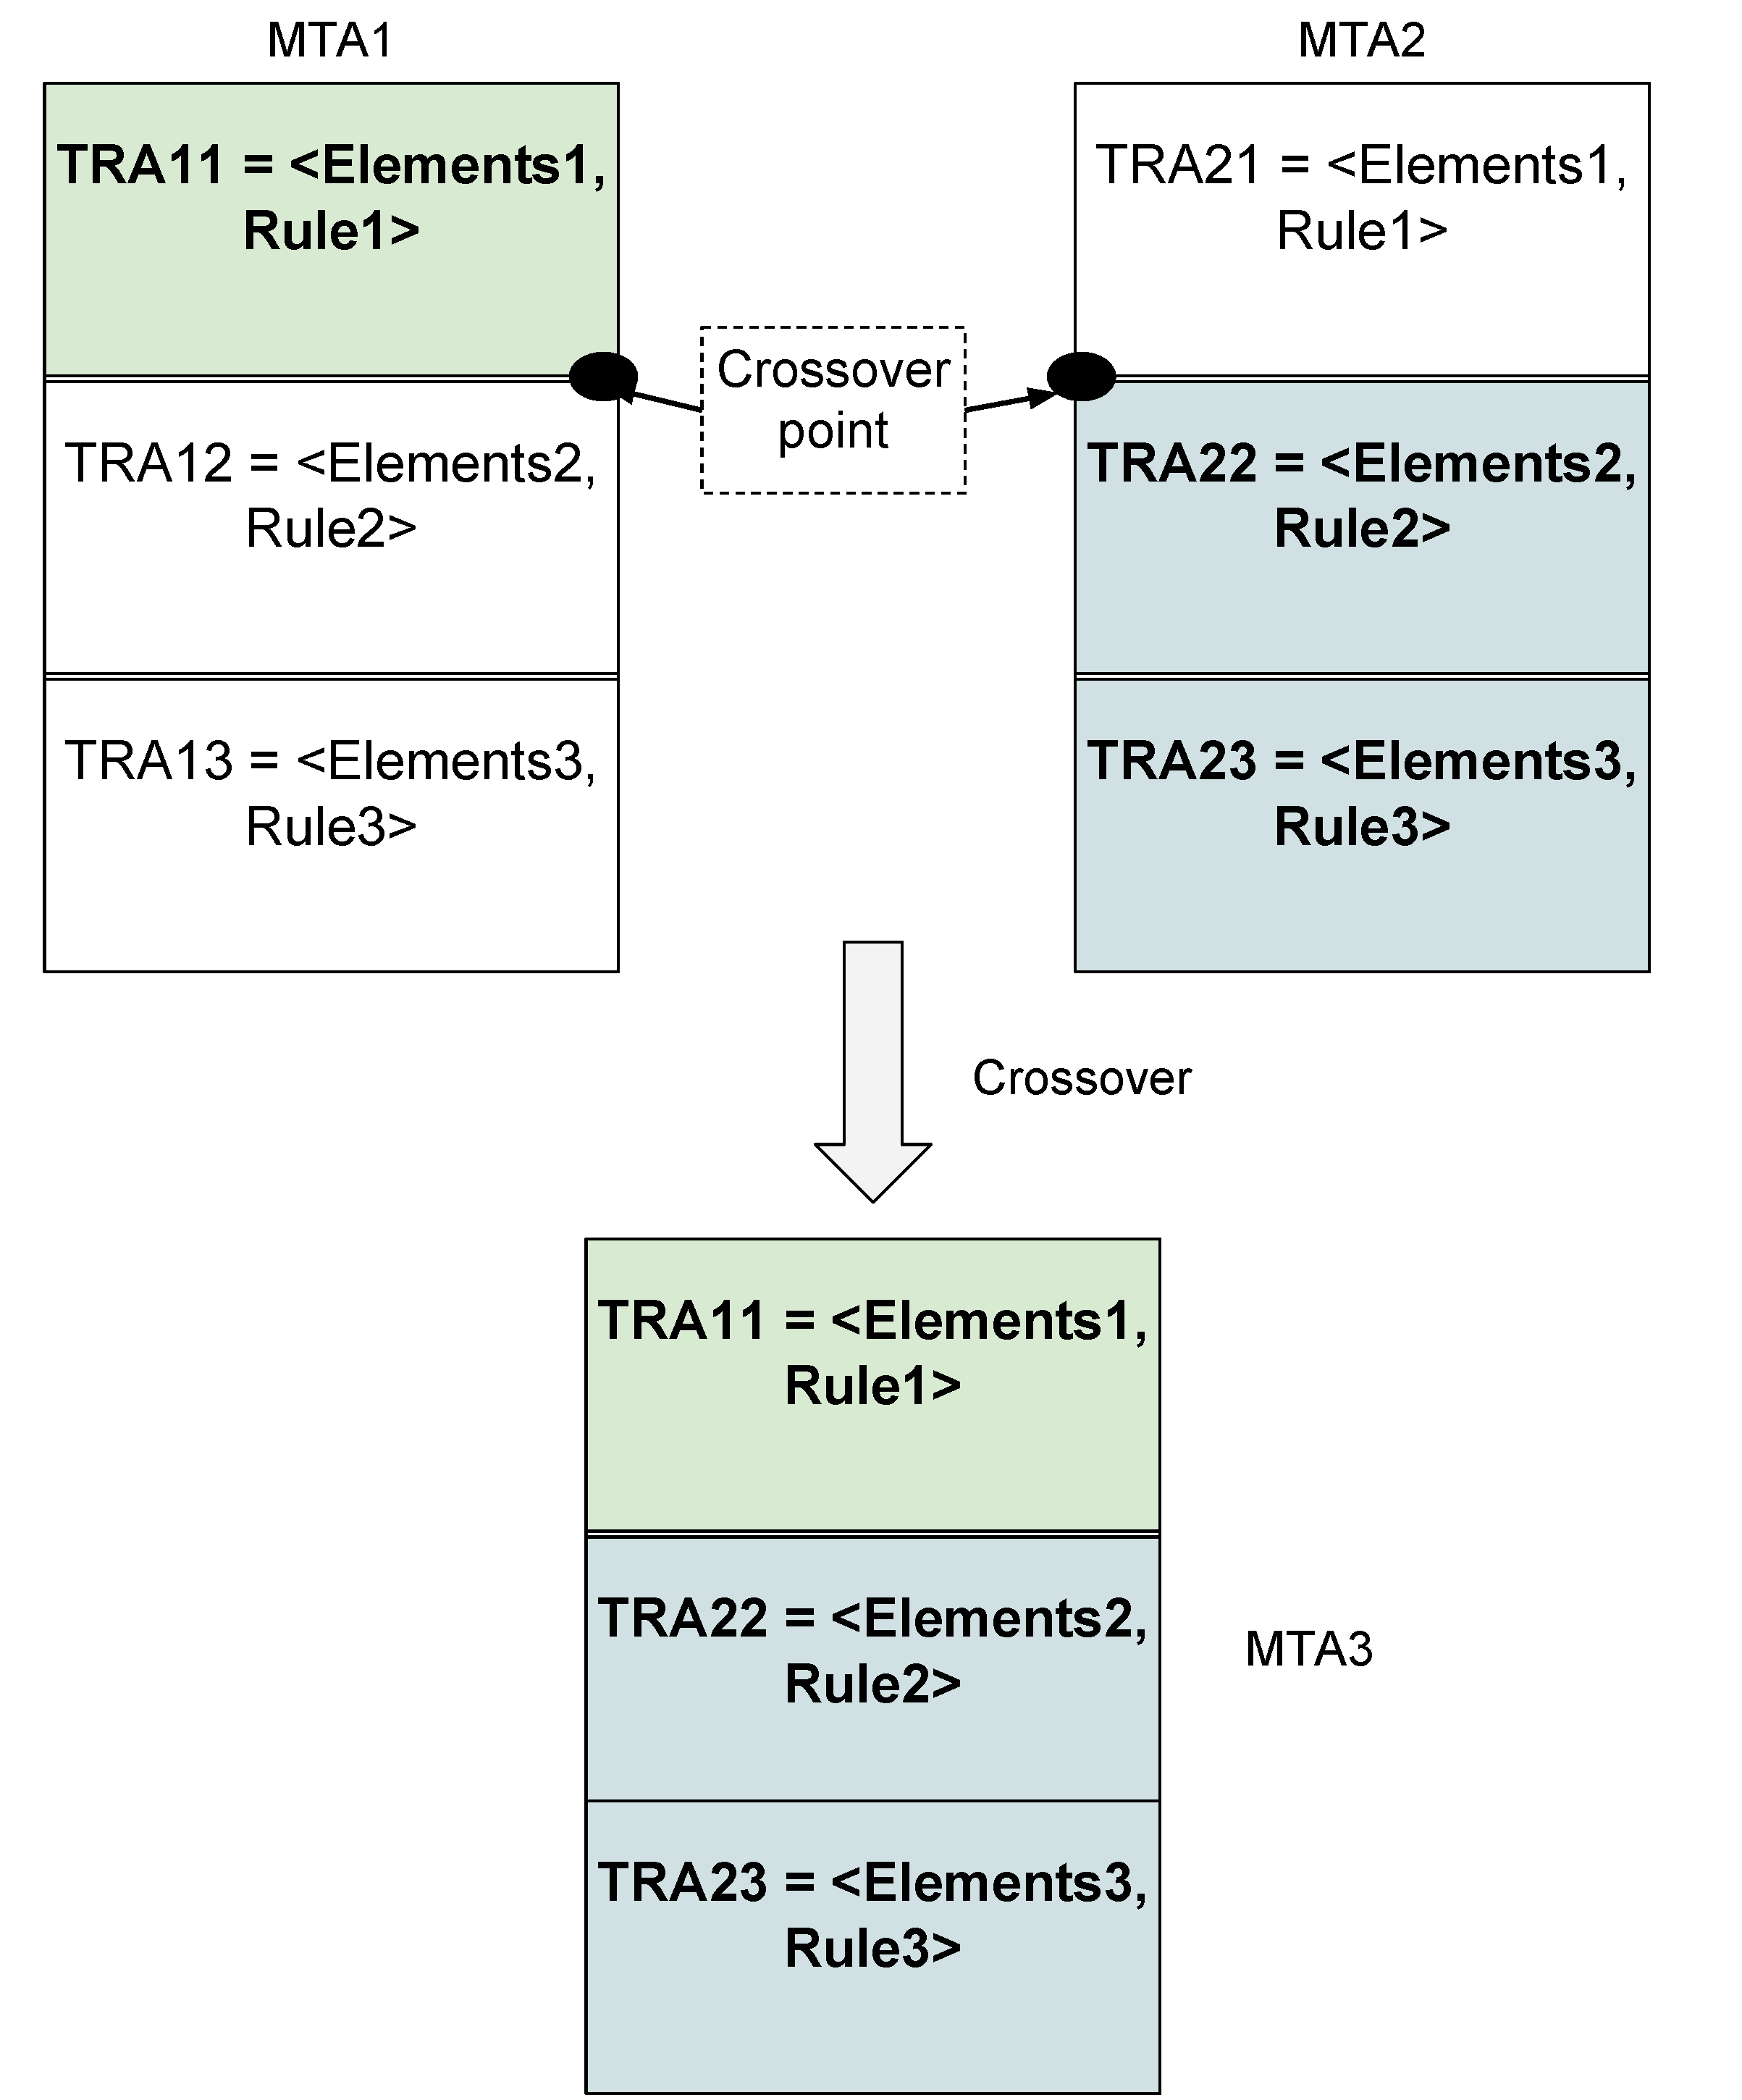
\includegraphics[width=3.49in]{crossover.pdf}
\caption{Crossover operator}
\label{crossover}
\end{figure}

\subsubsection{\textbf{Mutation}}
After performing the crossover, the obtained solutions could be mutated with a given mutation probability.
The mutation operator act on a single genome G1 to obtained a muted genome G11 acts as follows. The mutation operator selects a gene at random in the genome and changes its value. In Figure~\ref{mutation}, the third tile TRA13 is selected to mutate into TRA14 : we apply a different rule (i.e. rule4) to the set of selected elements.

%In the genetic algorithm used in the evolutionary design system above the genotypes consist of 1's and 0's, applying the mutation operator to a genotype of this kind switches a randomly selected 1 to a 0 or vice versa. 
%Indicating the core in the tile TRA as cs and ct as the core with which cs communicates most frequently, cs is remapped on a tile adjacent to Ts so as to reduce the distance between cs and ct . thus obtaining the mutated chromosome C0.


\begin{figure}[!t]
\centering
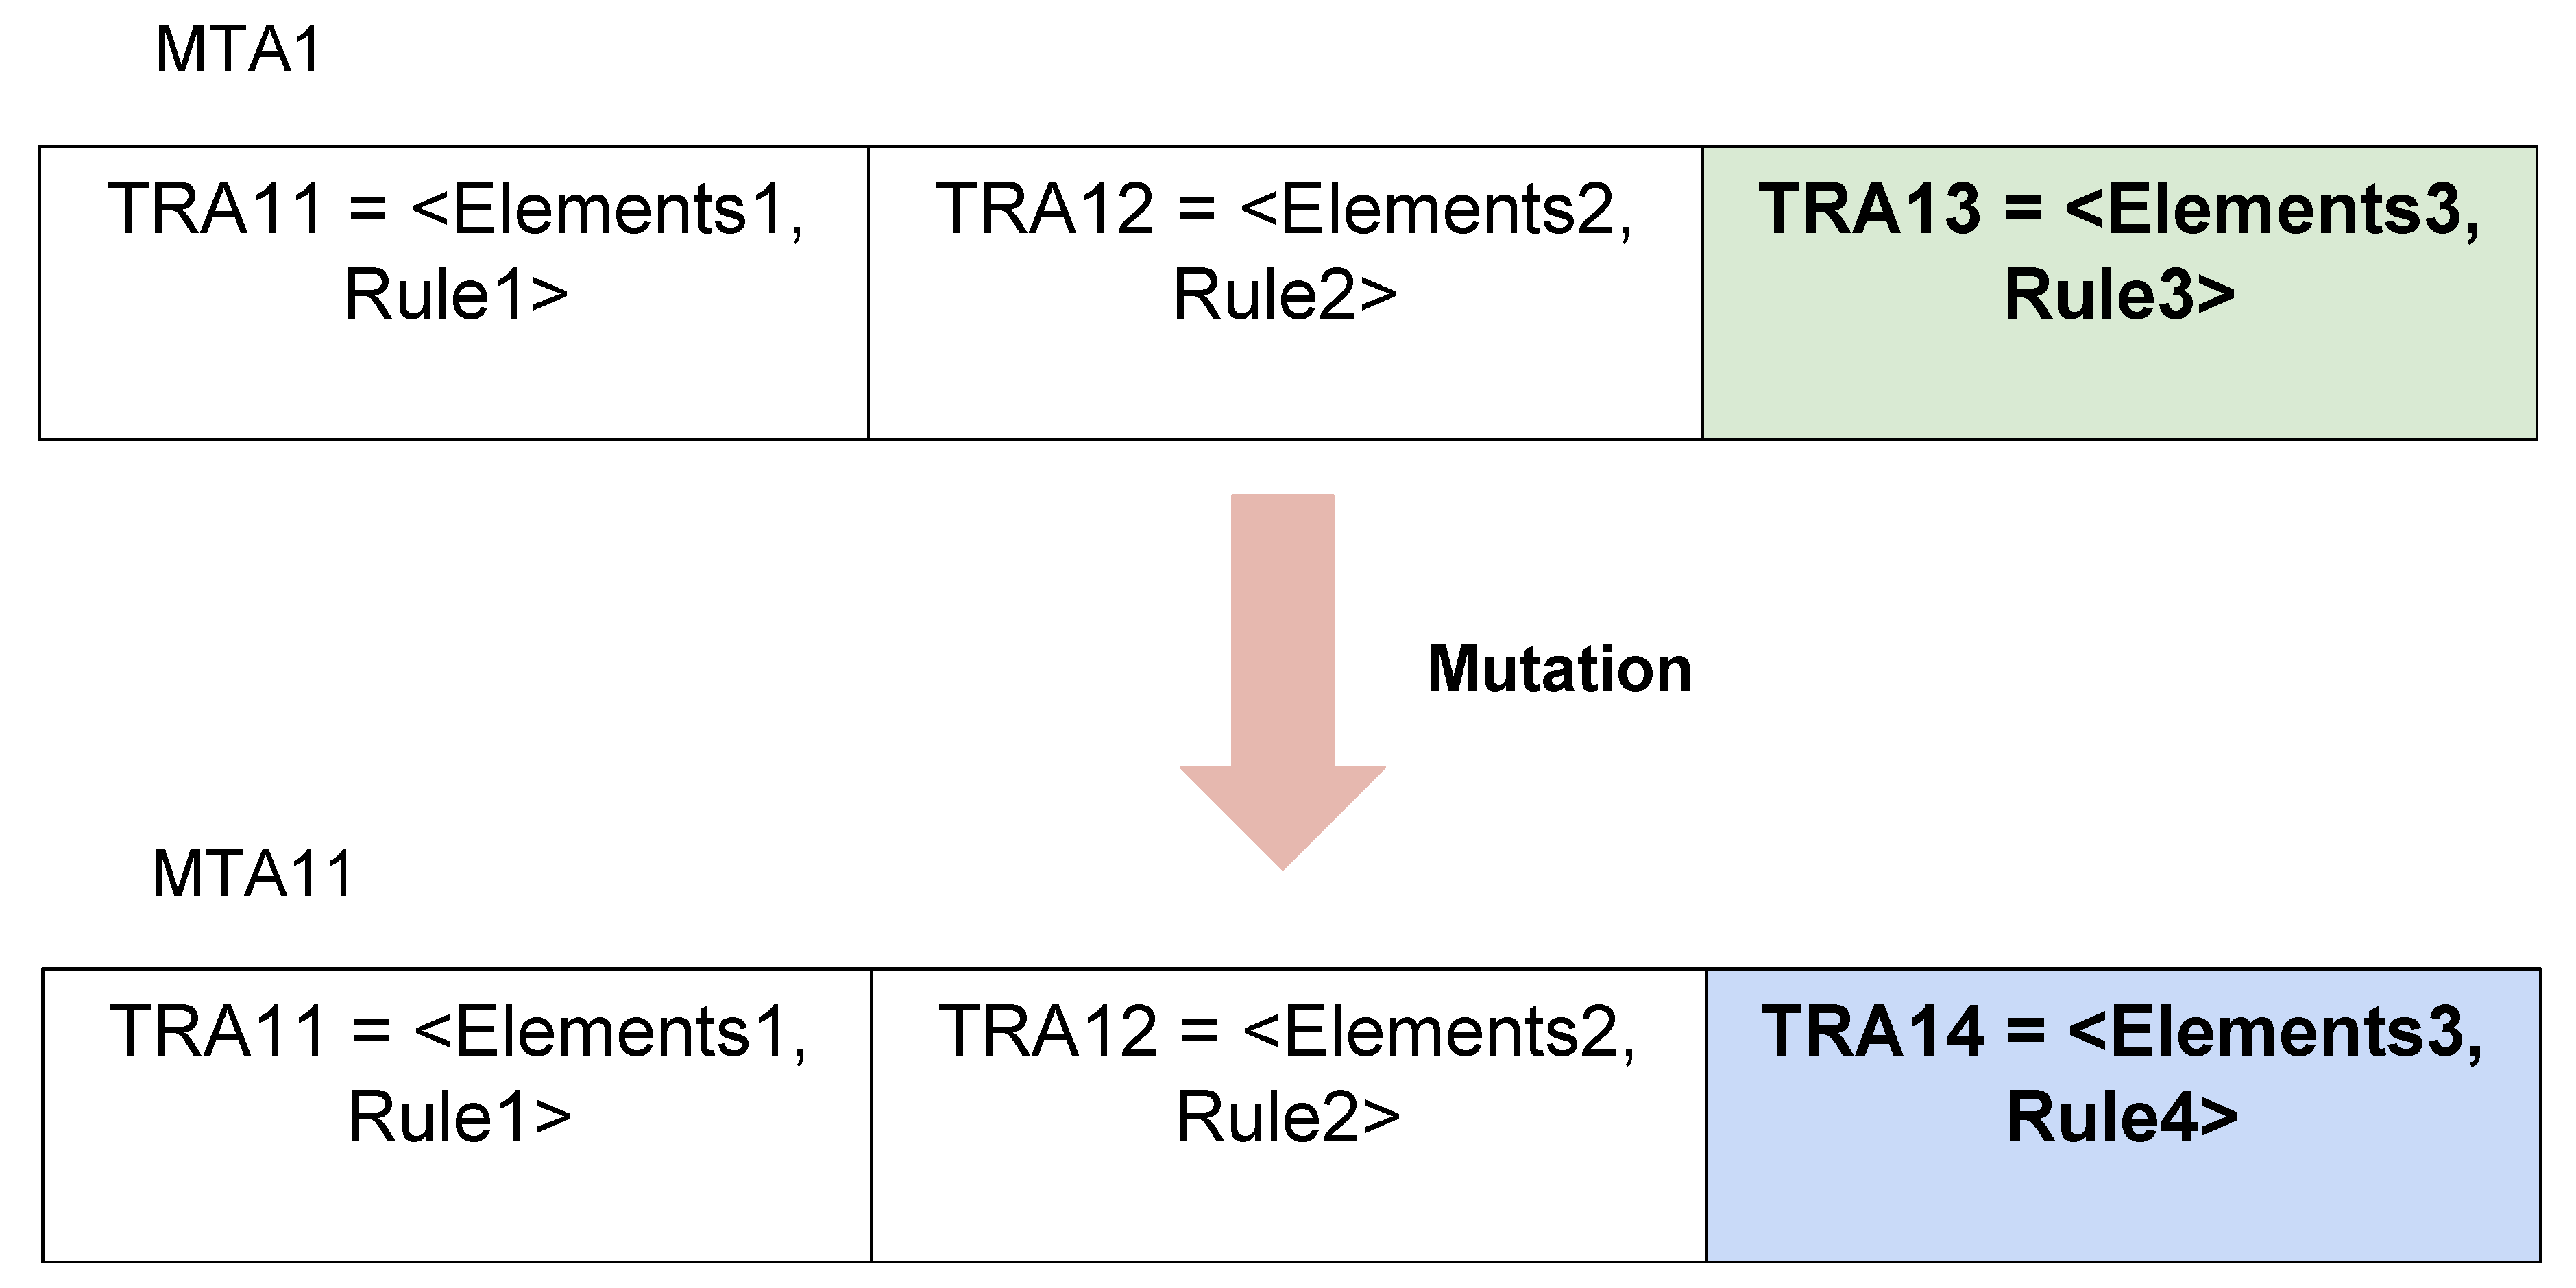
\includegraphics[width=3.49in]{mutation.pdf}
\caption{Mutation operator}
\label{mutation}
\end{figure}

%\subsection{\textbf{Use case}}
%Figure~\ref{nsgaDesign} gives an overview of the application of

%\begin{figure}[!t]
%\centering
%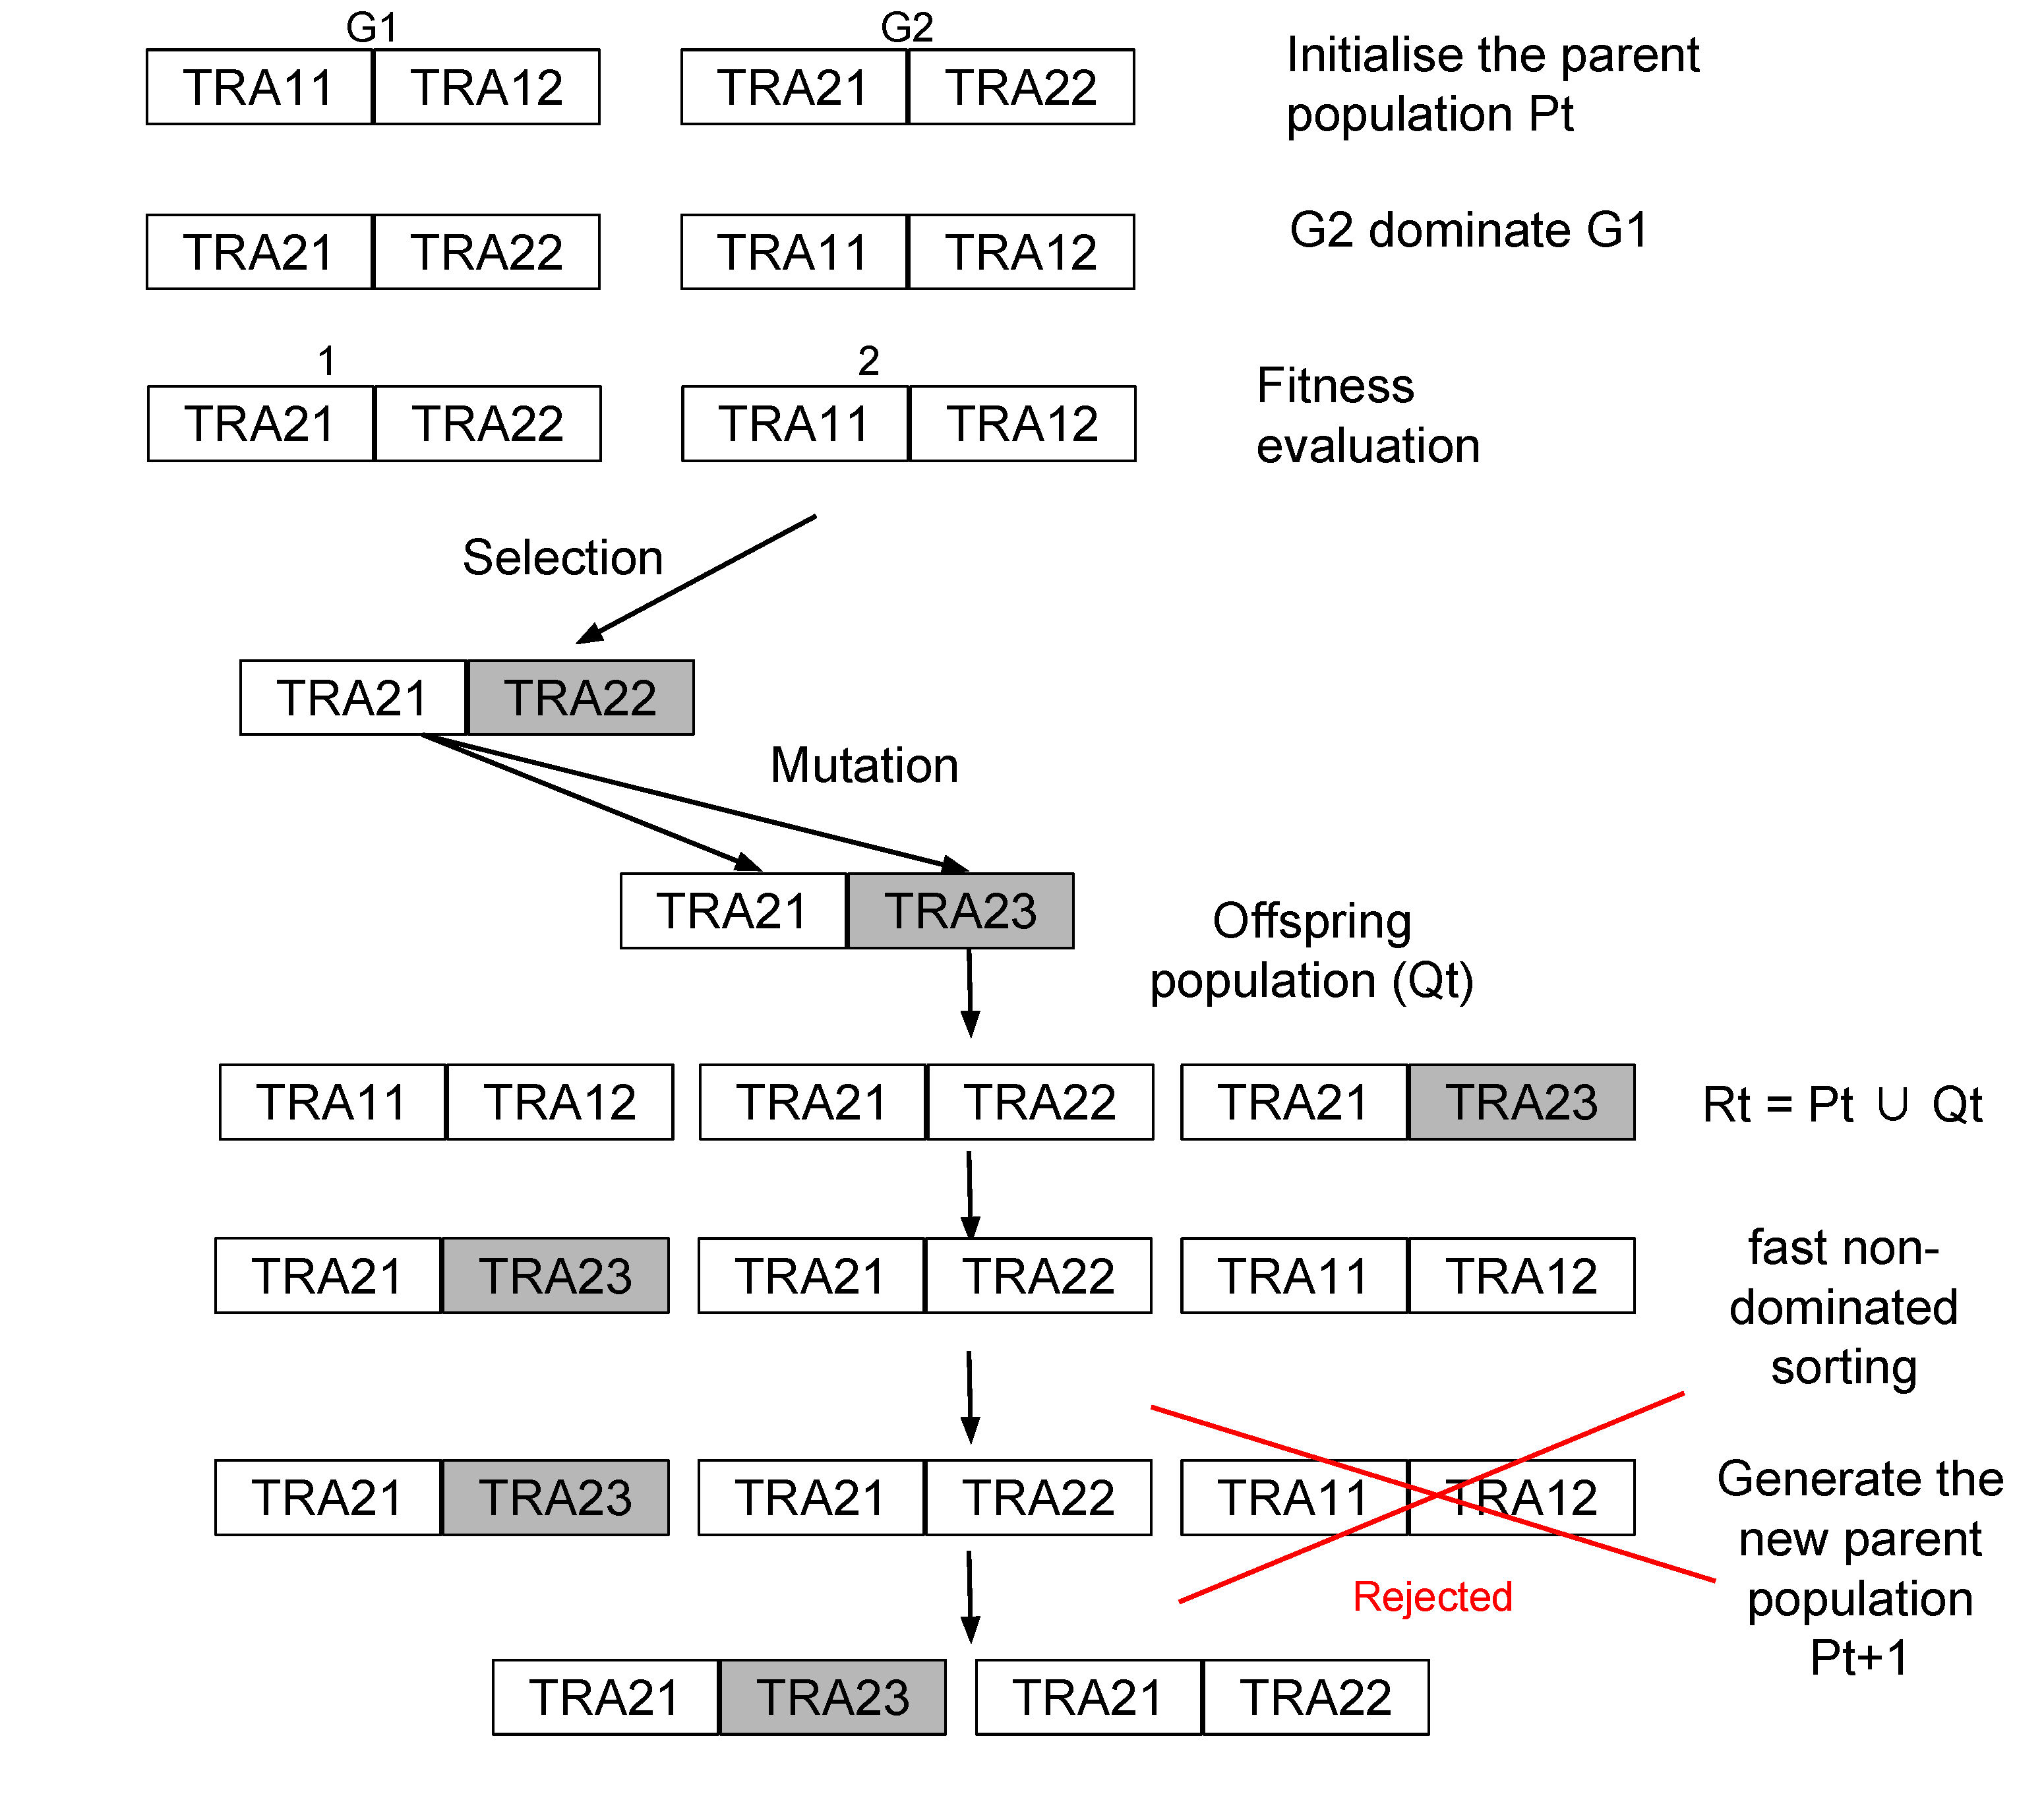
\includegraphics[width=3.49in]{nsgaDesign.pdf}
%\caption{Overview of the adaptation of NSGA-II}
%\label{nsgaDesign}
%\end{figure}


\section{Related Work}
\label{Related}
Our work is based on system performance prediction\cite{1291833} by using model transformations techniques and multi-objective metaheuristic optimization\cite{Coello98acomprehensive}.

Aleti et al.\cite{Gr5069138} have developed the ArchOpteryx framework. ArchOpteryx assists the system architects during the design to create architectures that meet non-functional properties by using multi-objective optimization strategies. Unlike this method, design alternatives are implemented as model transformations driven by NFP. Using model transformations help the design architects to (i) automating the system production; (ii) reusing architecture alternatives in other projects (or products) and (iii) solving the competition issue between NFP. Compared to DesignBots\cite{Diaz-Pace:2007:UPT:1784860.1784865}, in our method model transformations are not decomposed into subplans, each transformation is performed atomically.

Koziolek et al.\cite{Koziolek:2011:PAA:2000259.2000267} have developed the Peropteryx framework for improvement of system architecture models using a metaheuristic search guided by architectural tactics.

For the optimization of NFP another work consists at using a cyclic process\cite{Bosch99softwarearchitecture}. The benefit of this process is its simplicity. The process can be tailored to different non-functional properties by using specific evaluation methods and architecture transformations. But this process focuses on only one non-functional property at a time unlike us who take into account several properties at a same time (e.g. reliability, availability and response time).

\section{Conclusion}
\label{Conclu}
An architecture design method has been presented that explicitly addresses the NFP put on the architecture. The proposed approach aims at improving system architecture models using two mechanisms. On the one hand, model transformations compositions to formalize model design alternatives. On the other hand, an elitist multiple-objective optimisation algorithm to explore this design space.

The main benefits of this approach is to handle a large search spaces of quality optimization problems and to automate the identification of good architecture design alternatives. This will reduce development costs and improve the quality of the final system. Additionally this approach enables the ranking of design alternatives with respect to conflicting NFP and the possibility to reuse these alternatives in other projects or products by reusing model transformations.

In the future, we plan to integrate our approach in the framework RAMSES and evaluating our approach in more details quantitatively (i.e. experimenting it on a an industrial case study)\cite{greg}.

%Older works and experiments have shown that evolutionary algorithms and multiobjective optimization strategies can be used to identify Pareto-optimal or near Pareto-optimal architecture designs, which can be used as an input for architecture trade-off analysis techniques. 

%The main benefit of this approach is the ability to handle the large search spaces of quality optimization problems and to automate the identification of good architecture design alternatives. This will reduce development costs and improve the quality of the final system. Addition- ally this approach enables the ranking of design decisions (architectural refactorings) with respect to conflicting quality requirements.

\section{Acknowledgment}
This research work has been carried out under the leadership of the Technological Research Institute SystemX, and therefore granted with public funds within the scope of the French Program "Investissements d’Avenir".

\begin{thebibliography}{1}

\bibitem{Gr5069138}
A.~Aleti, S.~Bjornander, L.~Grunske, and I.~Meedeniya, ``Archeopterix: An
  extendable tool for architecture optimization of aadl models,'' in
  \emph{Model-Based Methodologies for Pervasive and Embedded Software, 2009.
  MOMPES '09. ICSE Workshop on}, May 2009, pp. 61--71.

\bibitem{1291833}
S.~Balsamo, A.~di~Marco, P.~Inverardi, and M.~Simeoni, ``Model-based
  performance prediction in software development: a survey,'' \emph{Software
  Engineering, IEEE Transactions on}, vol.~30, no.~5, pp. 295--310, May 2004.

\bibitem{Bosch99softwarearchitecture}
J.~Bosch, P.~Molin, J.~Bosch, and P.~Molin, ``Software architecture design:
  Evaluation and transformation,'' in \emph{In 1999 IEEE Engineering of
  Computer Based Systems Symposium. IEEE Computer Based Systems}, 1999, 
  pp. 4--10.

\bibitem{Coello98acomprehensive}
C.~A.~C. Coello, ``A comprehensive survey of evolutionary-based multiobjective
  optimization techniques,'' \emph{Knowledge and Information Systems}, vol.~1,
  pp. 269--308, 1998.

\bibitem{Deb:2002:FEM:2221359.2221582}
K.~Deb, A.~Pratap, S.~Agarwal, and T.~Meyarivan, ``A fast and elitist
  multiobjective genetic algorithm: Nsga-ii,'' \emph{Trans. Evol. Comp},
  vol.~6, no.~2, pp. 182--197, Apr. 2002. [Online]. Available:
  \url{http://dx.doi.org/10.1109/4235.996017}

\bibitem{Deb:2001:MOU:559152}
K.~Deb and D.~Kalyanmoy, \emph{Multi-Objective Optimization Using Evolutionary
  Algorithms}.\hskip 1em plus 0.5em minus 0.4em\relax New York, NY, USA: John
  Wiley \&amp; Sons, Inc., 2001.
 
\bibitem{Diaz-Pace:2007:UPT:1784860.1784865}
J.~A. D\'{\i}az-Pace and M.~R. Campo, ``Using planning techniques to assist
  quality-driven architectural design exploration,'' in \emph{Proceedings of
  the Quality of Software Architectures 3rd International Conference on
  Software Architectures, Components, and Applications}, ser. QoSA'07.\hskip
  1em plus 0.5em minus 0.4em\relax Berlin, Heidelberg: Springer-Verlag, 2007,
  pp. 33--52. [Online]. Available:
  \url{http://dl.acm.org/citation.cfm?id=1784860.1784865}

\bibitem{Johnsen1753}
A.~Johnsen and K.~Lundqvist, ``Developing dependable software-intensive
  systems: Aadl vs. east-adl,'' in \emph{Ada-Europe 2011}, A.~Romanovsky and
  T.~Vardanega, Eds.\hskip 1em plus 0.5em minus 0.4em\relax Springer-Verlag,
  June 2011, pp. 103--117. [Online]. Available:
  \url{http://www.es.mdh.se/publications/1753-}

\bibitem{Jouault:2005:TMA:2153686.2153705}
F.~Jouault and I.~Kurtev, ``Transforming models with atl,'' in
  \emph{Proceedings of the 2005 International Conference on Satellite Events at
  the MoDELS}, ser. MoDELS'05.\hskip 1em plus 0.5em minus 0.4em\relax Berlin,
  Heidelberg: Springer-Verlag, 2006, pp. 128--138. 
  [Online]. Available:  \url{http://dx.doi.org/10.1007/11663430_14}  
  
\bibitem{Kleppe2003}
A.~G. Kleppe, J.~Warmer, and W.~Bast, \emph{MDA Explained: The Model Driven
  Architecture: Practice and Promise}.\hskip 1em plus 0.5em minus 0.4em\relax
  Boston, MA, USA: Addison-Wesley Longman Publishing Co., Inc., 2003.

\bibitem{greg}
G.~Loniewski, E.~Borde, D.~Blouin and E.Insfran {\'{}}, ``An Automated Approach for Architectural Model
  Transformations,'' in \emph{Information Systems
  Development, 22nd International Conference, {ISD} 2013,
  Sevilla, Spain, September 2013. Proceedings}, 2013, pp. 295-306.
  [Online]. Available: \url{http://infres.enst.fr/~borde/isd2013loniewski.pdf}

\bibitem{Medvidovic}
N.~Medvidovic and R.~N. Taylor, ``A classification and comparison framework for
  software architecture description languages,'' \emph{IEEE Trans. Softw.
  Eng.}, vol.~26, no.~1, pp. 70--93, Jan. 2000. [Online]. Available:
  \url{http://dx.doi.org/10.1109/32.825767}

\bibitem{Srinivas94multiobjectiveoptimization}
N.~Srinivas and K.~Deb, ``Multiobjective optimization using nondominated
  sorting in genetic algorithms,'' \emph{Evolutionary Computation}, vol.~2, 
  pp. 221--248, 1994.

\bibitem{Tisi:conf/ecmdafa/TisiJFCB09}
M.~Tisi, F.~Jouault, P.~Fraternali, S.~Ceri, and J.~B{\'{e}}zivin, ``On the use
  of higher-order model transformations,'' in \emph{Model Driven Architecture -
  Foundations and Applications, 5th European Conference, {ECMDA-FA} 2009,
  Enschede, The Netherlands, June 23-26, 2009. Proceedings}, 2009, pp. 18--33.
  [Online]. Available: \url{http://dx.doi.org/10.1007/978-3-642-02674-4_3}

\bibitem{Yu:2001:CLA:502059.502038}
H.~Yu and A.~Vahdat, ``The costs and limits of availability for replicated
  services,'' \emph{SIGOPS Oper. Syst. Rev.}, vol.~35, no.~5, pp. 29--42, Oct.
  2001. [Online]. Available: 
  \url{http://doi.acm.org/10.1145/502059.502038}

\bibitem{Zitzler01spea2:improving}
E.~Zitzler, M.~Laumanns, and L.~Thiele, ``Spea2: Improving the strength pareto
  evolutionary algorithm,'' Tech. Rep., 2001.

\bibitem{Zitzler04indicatorbasedselection}
E.~Zitzler and S.~Künzli, ``Indicator-based selection in multiobjective
  search,'' in \emph{in Proc. 22nd International Conference on Information Systems
  Development (ISD 2013}.\hskip 1em plus 0.5em minus 0.4em\relax
  Springer, 2004, pp. 832--842.

\bibitem{Koziolek:2011:PAA:2000259.2000267}
A.~Koziolek, H.~Koziolek, and R.~Reussner, ``Peropteryx: Automated application
  of tactics in multi-objective software architecture optimization,'' in
  \emph{Proceedings of the Joint ACM SIGSOFT Conference -- QoSA and ACM SIGSOFT
  Symposium -- ISARCS on Quality of Software Architectures -- QoSA and
  Architecting Critical Systems -- ISARCS}, ser. QoSA-ISARCS '11.\hskip 1em
  plus 0.5em minus 0.4em\relax New York, NY, USA: ACM, 2011, pp. 33--42.
  [Online]. Available: \url{http://doi.acm.org/10.1145/2000259.2000267}

\end{thebibliography}

\end{document}